\documentclass{standalone}
\usepackage{tikz}
\usetikzlibrary{patterns, positioning}


\begin{document}
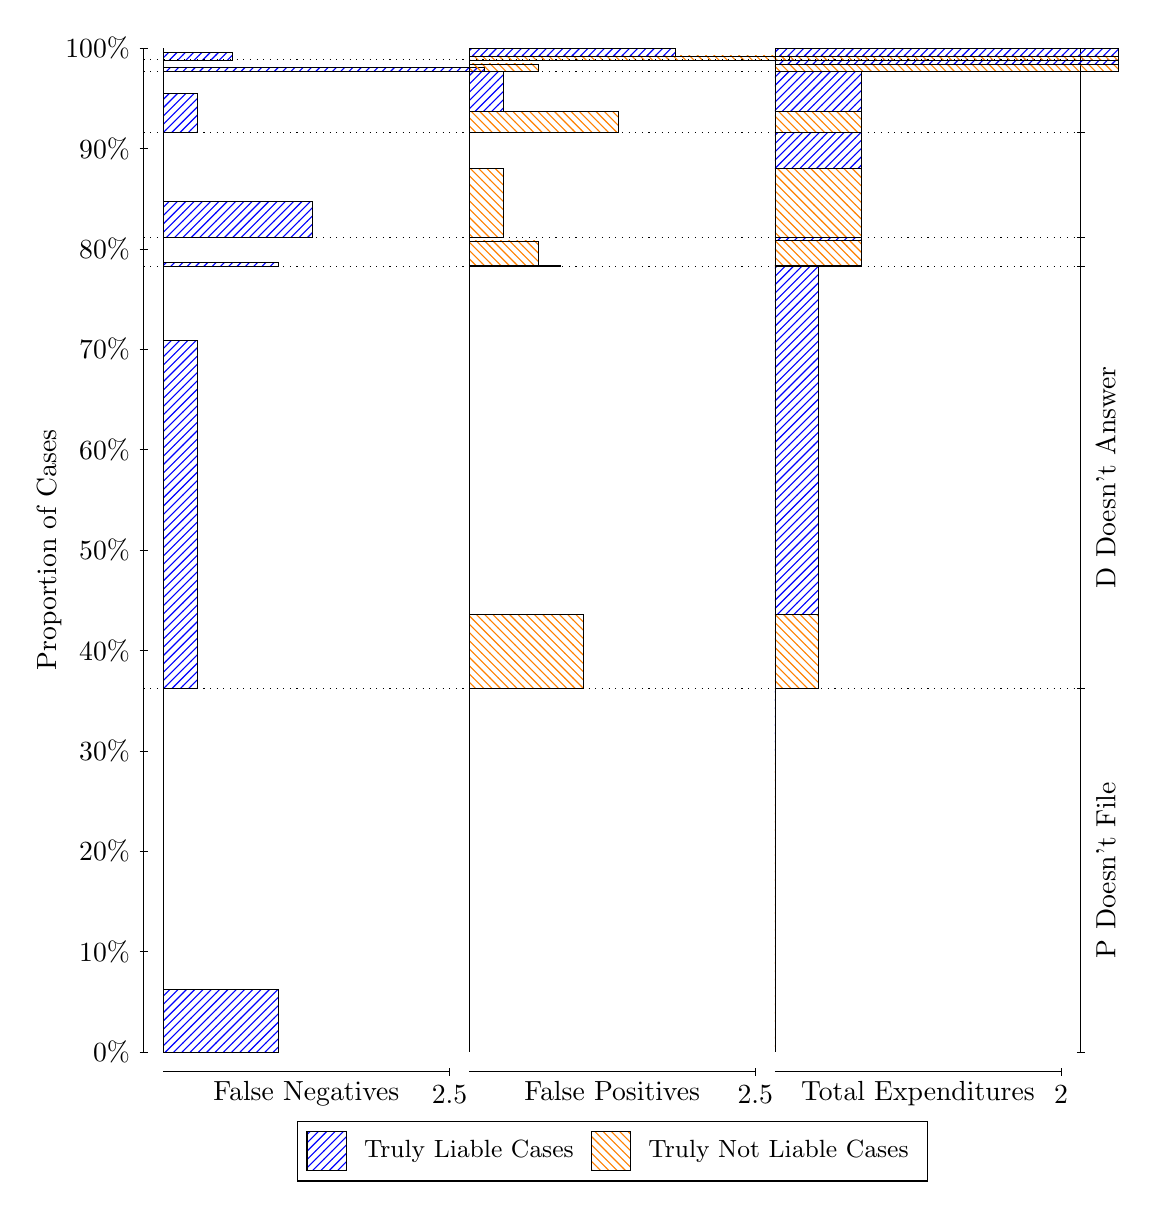
\begin{tikzpicture}
\draw[black, very thin] (1.5,1.75) -- (1.5,14.5);
\node[rotate=90, text=black, anchor=center] at (0.3, 8.125) {Proportion of Cases};
\draw[black, very thin] (1.45,1.75) -- (1.55,1.75);
\node[text=black, anchor=east] at (1.45, 1.75) {0\%};
\draw[black, very thin] (1.45,3.025) -- (1.55,3.025);
\node[text=black, anchor=east] at (1.45, 3.025) {10\%};
\draw[black, very thin] (1.45,4.3) -- (1.55,4.3);
\node[text=black, anchor=east] at (1.45, 4.3) {20\%};
\draw[black, very thin] (1.45,5.575) -- (1.55,5.575);
\node[text=black, anchor=east] at (1.45, 5.575) {30\%};
\draw[black, very thin] (1.45,6.85) -- (1.55,6.85);
\node[text=black, anchor=east] at (1.45, 6.85) {40\%};
\draw[black, very thin] (1.45,8.125) -- (1.55,8.125);
\node[text=black, anchor=east] at (1.45, 8.125) {50\%};
\draw[black, very thin] (1.45,9.4) -- (1.55,9.4);
\node[text=black, anchor=east] at (1.45, 9.4) {60\%};
\draw[black, very thin] (1.45,10.675) -- (1.55,10.675);
\node[text=black, anchor=east] at (1.45, 10.675) {70\%};
\draw[black, very thin] (1.45,11.95) -- (1.55,11.95);
\node[text=black, anchor=east] at (1.45, 11.95) {80\%};
\draw[black, very thin] (1.45,13.225) -- (1.55,13.225);
\node[text=black, anchor=east] at (1.45, 13.225) {90\%};
\draw[black, very thin] (1.45,14.5) -- (1.55,14.5);
\node[text=black, anchor=east] at (1.45, 14.5) {100\%};

\draw[black, very thin] (13.4,1.75) -- (13.4,14.5);
\draw[black, very thin] (13.35,1.75) -- (13.45,1.75);
\node[anchor=west] at (13.35, 1.75) {};
\draw[black, very thin] (13.35,6.3685) -- (13.45,6.3685);
\node[anchor=west] at (13.35, 6.3685) {};
\draw[black, very thin] (13.35,11.73) -- (13.45,11.73);
\node[anchor=west] at (13.35, 11.73) {};
\draw[black, very thin] (13.35,12.098) -- (13.45,12.098);
\node[anchor=west] at (13.35, 12.098) {};
\draw[black, very thin] (13.35,13.426) -- (13.45,13.426);
\node[anchor=west] at (13.35, 13.426) {};
\draw[black, very thin] (13.35,14.199) -- (13.45,14.199);
\node[anchor=west] at (13.35, 14.199) {};
\draw[black, very thin] (13.35,14.35) -- (13.45,14.35);
\node[anchor=west] at (13.35, 14.35) {};
\draw[black, very thin] (13.35,14.5) -- (13.45,14.5);
\node[anchor=west] at (13.35, 14.5) {};

\draw[black, very thin, pattern color=blue, pattern=north east lines] (1.75,1.75) rectangle (3.2033,2.545);
\draw[black, very thin, pattern color=orange, pattern=north west lines] (1.75,2.545) rectangle (1.75,6.3685);
\draw[black, very thin, pattern color=blue, pattern=north east lines] (1.75,6.3685) rectangle (2.186,10.792);
\draw[black, very thin, pattern color=orange, pattern=north west lines] (1.75,10.792) rectangle (1.75,11.73);
\draw[black, very thin, pattern color=blue, pattern=north east lines] (1.75,11.73) rectangle (3.2033,11.773);
\draw[black, very thin, pattern color=blue, pattern=north east lines] (1.75,11.773) rectangle (2.9127,11.778);
\draw[black, very thin, pattern color=orange, pattern=north west lines] (1.75,11.778) rectangle (1.75,12.098);
\draw[black, very thin, pattern color=blue, pattern=north east lines] (1.75,12.098) rectangle (3.6393,12.557);
\draw[black, very thin, pattern color=orange, pattern=north west lines] (1.75,12.557) rectangle (1.75,13.426);
\draw[black, very thin, pattern color=blue, pattern=north east lines] (1.75,13.426) rectangle (2.186,13.926);
\draw[black, very thin, pattern color=orange, pattern=north west lines] (1.75,13.926) rectangle (1.75,14.199);
\draw[black, very thin, pattern color=blue, pattern=north east lines] (1.75,14.199) rectangle (5.8193,14.25);
\draw[black, very thin, pattern color=orange, pattern=north west lines] (1.75,14.25) rectangle (1.75,14.35);
\draw[black, very thin, pattern color=blue, pattern=north east lines] (1.75,14.35) rectangle (2.622,14.449);
\draw[black, very thin, pattern color=orange, pattern=north west lines] (1.75,14.449) rectangle (1.75,14.5);
\draw[black, very thin, pattern color=orange, pattern=north west lines] (5.6333,1.75) rectangle (5.6333,5.5736);
\draw[black, very thin, pattern color=blue, pattern=north east lines] (5.6333,5.5736) rectangle (5.6333,6.3685);
\draw[black, very thin, pattern color=orange, pattern=north west lines] (5.6333,6.3685) rectangle (7.0867,7.3067);
\draw[black, very thin, pattern color=blue, pattern=north east lines] (5.6333,7.3067) rectangle (5.6333,11.73);
\draw[black, very thin, pattern color=orange, pattern=north west lines] (5.6333,11.73) rectangle (6.796,11.735);
\draw[black, very thin, pattern color=orange, pattern=north west lines] (5.6333,11.735) rectangle (6.5053,12.051);
\draw[black, very thin, pattern color=blue, pattern=north east lines] (5.6333,12.051) rectangle (5.6333,12.098);
\draw[black, very thin, pattern color=orange, pattern=north west lines] (5.6333,12.098) rectangle (6.0693,12.967);
\draw[black, very thin, pattern color=blue, pattern=north east lines] (5.6333,12.967) rectangle (5.6333,13.426);
\draw[black, very thin, pattern color=orange, pattern=north west lines] (5.6333,13.426) rectangle (7.5227,13.699);
\draw[black, very thin, pattern color=blue, pattern=north east lines] (5.6333,13.699) rectangle (6.0693,14.199);
\draw[black, very thin, pattern color=orange, pattern=north west lines] (5.6333,14.199) rectangle (6.5053,14.299);
\draw[black, very thin, pattern color=blue, pattern=north east lines] (5.6333,14.299) rectangle (5.6333,14.35);
\draw[black, very thin, pattern color=orange, pattern=north west lines] (5.6333,14.35) rectangle (9.7027,14.401);
\draw[black, very thin, pattern color=blue, pattern=north east lines] (5.6333,14.401) rectangle (8.2493,14.5);
\draw[black, very thin, pattern color=orange, pattern=north west lines] (9.5167,1.75) rectangle (9.5167,5.5736);
\draw[black, very thin, pattern color=blue, pattern=north east lines] (9.5167,5.5736) rectangle (9.5167,6.3685);
\draw[black, very thin, pattern color=orange, pattern=north west lines] (9.5167,6.3685) rectangle (10.062,7.3067);
\draw[black, very thin, pattern color=blue, pattern=north east lines] (9.5167,7.3067) rectangle (10.062,11.73);
\draw[black, very thin, pattern color=orange, pattern=north west lines] (9.5167,11.73) rectangle (10.607,11.735);
\draw[black, very thin, pattern color=blue, pattern=north east lines] (9.5167,11.735) rectangle (10.607,11.74);
\draw[black, very thin, pattern color=orange, pattern=north west lines] (9.5167,11.74) rectangle (10.607,12.056);
\draw[black, very thin, pattern color=blue, pattern=north east lines] (9.5167,12.056) rectangle (10.607,12.098);
\draw[black, very thin, pattern color=orange, pattern=north west lines] (9.5167,12.098) rectangle (10.607,12.967);
\draw[black, very thin, pattern color=blue, pattern=north east lines] (9.5167,12.967) rectangle (10.607,13.426);
\draw[black, very thin, pattern color=orange, pattern=north west lines] (9.5167,13.426) rectangle (10.607,13.699);
\draw[black, very thin, pattern color=blue, pattern=north east lines] (9.5167,13.699) rectangle (10.607,14.199);
\draw[black, very thin, pattern color=orange, pattern=north west lines] (9.5167,14.199) rectangle (13.877,14.299);
\draw[black, very thin, pattern color=blue, pattern=north east lines] (9.5167,14.299) rectangle (13.877,14.35);
\draw[black, very thin, pattern color=orange, pattern=north west lines] (9.5167,14.35) rectangle (13.877,14.401);
\draw[black, very thin, pattern color=blue, pattern=north east lines] (9.5167,14.401) rectangle (13.877,14.5);
\draw[black, dotted] (1.5,6.3685) -- (13.4,6.3685);
\draw[black, dotted] (1.5,11.73) -- (13.4,11.73);
\draw[black, dotted] (1.5,12.098) -- (13.4,12.098);
\draw[black, dotted] (1.5,13.426) -- (13.4,13.426);
\draw[black, dotted] (1.5,14.199) -- (13.4,14.199);
\draw[black, dotted] (1.5,14.35) -- (13.4,14.35);
\draw[black, very thin] (1.75,1.5) -- (5.3833,1.5);
\node[text=black, anchor=north] at (3.5667, 1.5) {False Negatives};
\draw[black, very thin] (5.3833,1.45) -- (5.3833,1.55);
\node[text=black, anchor=north] at (5.3833, 1.45) {2.5};

\draw[black, very thin] (5.6333,1.5) -- (9.2667,1.5);
\node[text=black, anchor=north] at (7.45, 1.5) {False Positives};
\draw[black, very thin] (9.2667,1.45) -- (9.2667,1.55);
\node[text=black, anchor=north] at (9.2667, 1.45) {2.5};

\draw[black, very thin] (9.5167,1.5) -- (13.15,1.5);
\node[text=black, anchor=north] at (11.333, 1.5) {Total Expenditures};
\draw[black, very thin] (13.15,1.45) -- (13.15,1.55);
\node[text=black, anchor=north] at (13.15, 1.45) {2};

\node[text=black, centered, rotate=90] at (13.72, 4.0593) {P Doesn't File};
\node[text=black, centered, rotate=90] at (13.72, 9.0494) {D Doesn't Answer};






\draw (7.449999999999999,1.5) node[draw=none] (baseCoordinate) {};
\begin{scope}[align=center]
        \matrix[scale=0.5, draw=black, below=0.5cm of baseCoordinate, nodes={draw}, column sep=0.1cm]{
            \node[rectangle, draw, minimum width=0.5cm, minimum height=0.5cm, pattern color=blue, pattern=north east lines] {}; &
            \node[draw=none, font=\small, text=black] (B) {Truly Liable Cases}; &
            \node[rectangle, draw, minimum width=0.5cm, minimum height=0.5cm, pattern color=orange, pattern=north west lines] {}; &
            \node[draw=none, font=\small, text=black] (B) {Truly Not Liable Cases}; \\
            };
\end{scope}

\end{tikzpicture}
\end{document}